\section{Modulación AM}

Para el circuito de la figura entregada:

\begin{figure}[ht!]
    \centering
    \begin{tikzpicture}
        % Paths, nodes and wires:
        \draw (1, 5.5) to[sinusoidal voltage source, l={$V_i$}, label distance=0.02cm] (1, 3.5);
        \draw (4, 3) to[sinusoidal voltage source, l={$V_c$}, label distance=0.02cm] (4, 1);
        \draw (2, 6) to[american resistor, l={$R$}, label distance=0.02cm] (5, 6);
        \draw node[op amp] at (6.19, 5.51) {};
        \draw (5, 5.02) to[american resistor, l={$R/2$}, label distance=0.02cm] (2, 5);
        \draw (1, 5.5) -| (2, 6);
        \draw (2, 5.5) -| (2, 5);
        \draw (5, 7) to[american resistor, l={$R$}, label distance=0.02cm] (7, 7);
        \draw (5, 7) -| (5, 6);
        \draw (7, 7) -| (7.38, 5.51);
        \draw node[nmos] at (5, 2.98) {};
        \draw (5, 5) -| (5, 3.75);
        \draw (5, 2.21) -| (5, 1);
        \draw node[sground] at (5, 1) {};
        \draw node[sground] at (4, 1) {};
        \draw node[sground] at (1, 3.5) {};
        \draw (7.38, 5.51) -| (8, 5.5);
        \draw node[ocirc] (N1) at (8, 5.5) {} node[anchor=west] at (N1.east){$V_o$};
        \draw node[circ] (N2) at (5, 5) {} node[anchor=south east] at (N2.north west){$V_+$};
        \draw node[circ] (N3) at (5, 6) {} node[anchor=south east] at (N3.north west){$V_-$};
    \end{tikzpicture}
    \caption{Circuito de Modulación AM}
    \label{fig:am_mod_ckt}
\end{figure}

\subsection{Análisis Teórico}
Se puede hacer un análisis según el estado del transistor, abierto y cerrado.

\paragraph{Transistor abierto} ($V_c$ Low)

Se tiene una fuente conectada a ambas entradas del op-amp. En el caso de $V_+$, como no fluye corriente, va a ser igual a $V_i$, lo que significa (por cortocircuito virtual) que $V_- = V_i$. De esta manera, sabemos que no fluye corriente a través de $R$ (ninguna), entonces $V_o$ debe ser igual a $V_i$.
\paragraph{Transistor cerrado} ($V_c$ High)

Como el transistor cerrado significa un cortocircuito, se ve que $V_+ = 0$ (tierra) y de esta manera $V_- = 0$ y la corriente a través de $R$ es $\frac{V_i}{R}$, por lo que $V_o = -V_i$.

De esta manera, cuando $V_c^H$, $V_o = -V_i$, y cuando $V_c^L$, $V_o = V_i$.

La onda cuadrada $V_c$ segmenta así la señal de entrada $V_i$, y el amplificador operacional amplifica los segmentos cuando el interruptor está cerrado. El resultado $V_o$ es una versión pulsada de $V_i$, donde la amplitud varía con el ciclo de trabajo de $V_c$. Este proceso de segmentación y amplificación es la base de la Modulación por Amplitud (AM), ya que la envolvente de $V_o$ sigue la amplitud de $V_i$ modulada por la acción de conmutación de $V_c$.

\subsubsection{Mecanismo de Generación AM}

La modulación AM consiste en variar la amplitud de una señal portadora (en este caso, la acción de conmutación de $V_c$) en proporción a la señal de mensaje $V_i$.

La onda cuadrada $V_c$ actúa como señal portadora, siendo su frecuencia la que determina la tasa de modulación. Cuando el interruptor está cerrado, $V_i$ es muestreada y amplificada, creando una envolvente de amplitud que refleja la forma de onda de $V_i$.

La salida $V_o$ contiene la frecuencia portadora (proveniente de $V_c$) y bandas laterales resultantes de la modulación de $V_i$. Para componentes ideales, el espectro incluye la frecuencia portadora y las bandas laterales superior e inferior centradas alrededor de ella.

\subsubsection{Relación de Frecuencias}

Cualitativamente, la frecuencia de $V_c$ (frecuencia portadora, $f_c$) debe ser significativamente mayor que la frecuencia de $V_i$ (frecuencia del mensaje, $f_m$). Típicamente, se cumple que $f_c \gg f_m$ (por ejemplo, $f_c$ debería ser al menos 10 veces $f_m$) para asegurar un muestreo y reconstrucción adecuados de la señal modulada sin distorsión significativa.

Esto garantiza que la acción de conmutación muestree adecuadamente a $V_i$, permitiendo que la envolvente represente con precisión la señal de entrada.

\subsubsection{Roles en la Modulación}

\begin{itemize}
    \item \textbf{Señal de entrada $V_i$}: Es la señal moduladora (mensaje), como una onda senoidal o señal de audio, cuyas variaciones de amplitud se imponen sobre la portadora.
    \item \textbf{Pulso de control $V_c$}: Actúa como señal portadora, controlando la conmutación para segmentar $V_i$ y así crear la salida modulada en amplitud.
\end{itemize}

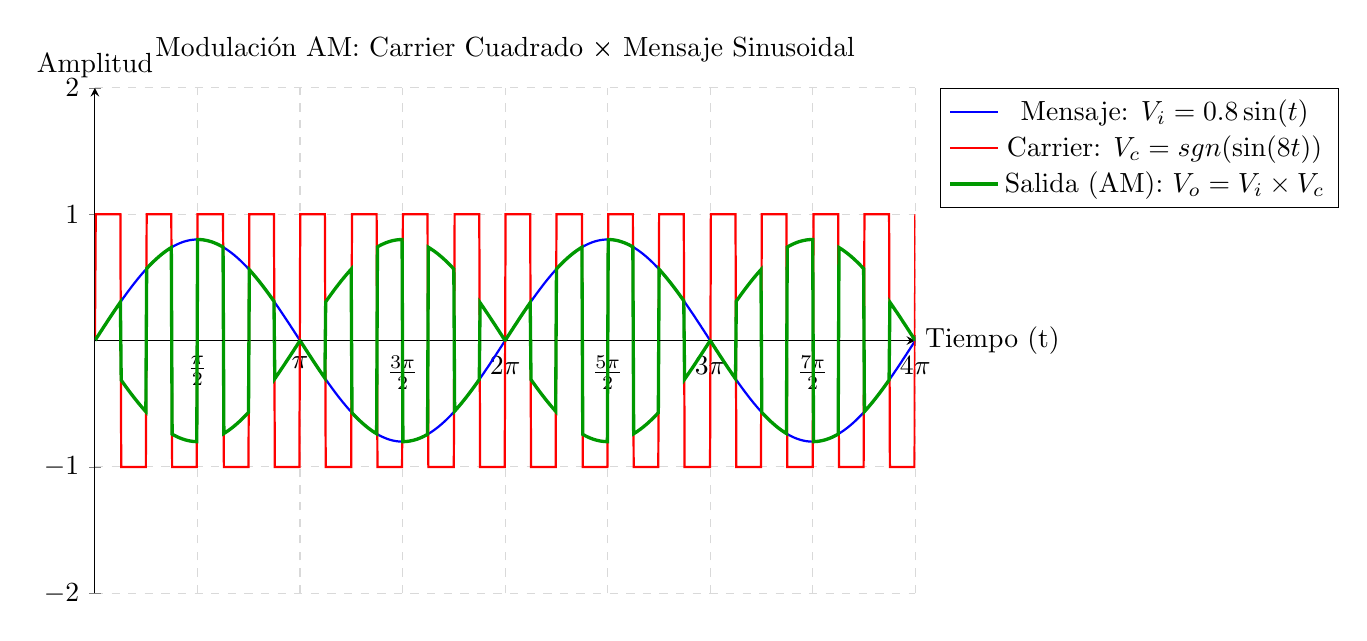
\begin{tikzpicture}
    \begin{axis}[
            width=12cm,
            height=8cm,
            xlabel={Tiempo (t)},
            ylabel={Amplitud},
            title={Modulación AM: Carrier Cuadrado × Mensaje Sinusoidal},
            grid=major,
            grid style={dashed,gray!30},
            legend pos=outer north east,
            samples=500,
            domain=0:4*pi,
            xmin=0, xmax=4*pi,
            ymin=-2, ymax=2,
            xtick={0, pi/2, pi, 3*pi/2, 2*pi, 5*pi/2, 3*pi, 7*pi/2, 4*pi},
            xticklabels={0, $\frac{\pi}{2}$, $\pi$, $\frac{3\pi}{2}$, $2\pi$, $\frac{5\pi}{2}$, $3\pi$, $\frac{7\pi}{2}$, $4\pi$},
            axis lines=center,
            every axis x label/.style={at={(current axis.right of origin)},anchor=west},
            every axis y label/.style={at={(current axis.above origin)},anchor=south},
        ]

        % Message signal (sine wave)
        \addplot[blue, thick, smooth] {0.8*sin(deg(x))};
        \addlegendentry{Mensaje: $V_i = 0.8\sin(t)$}

        % Square wave carrier (using sign function approximation)
        \addplot[red, thick, samples=1000] {sign(sin(deg(8*x)))};
        \addlegendentry{Carrier: $V_c = \text{sgn}(\sin(8t))$}

        % AM modulated signal (product)
        \addplot[green!60!black, very thick, samples=1000] {0.8*sin(deg(x))*sign(sin(deg(8*x)))};
        \addlegendentry{Salida (AM): $V_o = V_i \times V_c$}

        % Zero reference line
        \addplot[black, dotted, thin] {0};

    \end{axis}
\end{tikzpicture}

\vspace{1cm}

% Add mathematical explanation
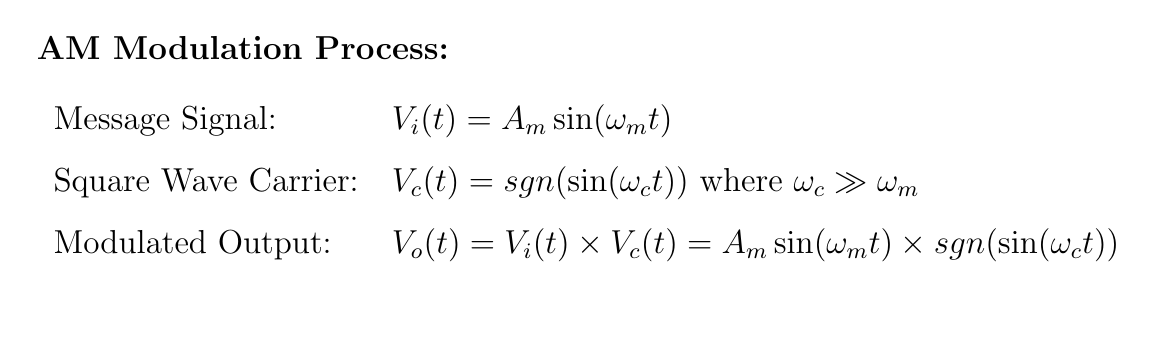
\begin{tikzpicture}
    \node[align=left, font=\large] at (0,0) {
        \textbf{AM Modulation Process:}\\[0.5cm]
        \begin{tabular}{ll}
            Message Signal:      & $V_i(t) = A_m \sin(\omega_m t)$                                                            \\[0.3cm]
            Square Wave Carrier: & $V_c(t) = \text{sgn}(\sin(\omega_c t))$ where $\omega_c \gg \omega_m$                      \\[0.3cm]
            Modulated Output:    & $V_o(t) = V_i(t) \times V_c(t) = A_m \sin(\omega_m t) \times \text{sgn}(\sin(\omega_c t))$ \\[0.5cm]
        \end{tabular}
    };
\end{tikzpicture}

Ahora, si tomamos un \textit{carrier} de baja frecuencia:

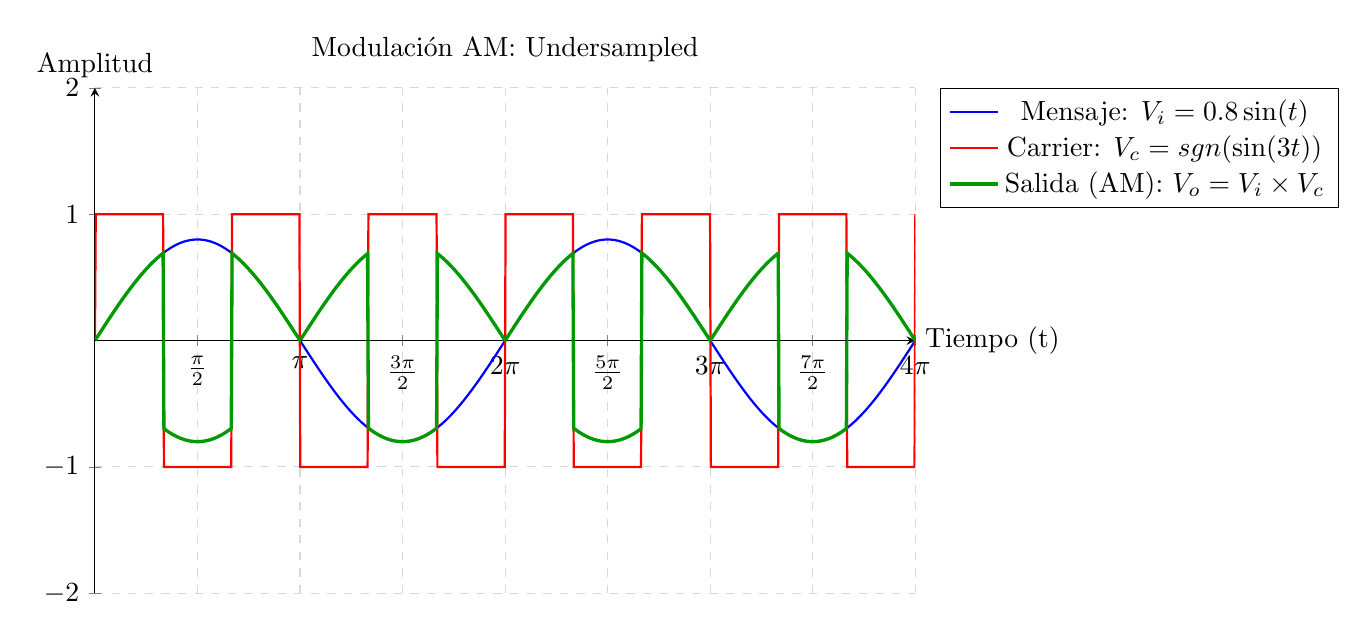
\begin{tikzpicture}
    \begin{axis}[
            width=12cm,
            height=8cm,
            xlabel={Tiempo (t)},
            ylabel={Amplitud},
            title={Modulación AM: Undersampled},
            grid=major,
            grid style={dashed,gray!30},
            legend pos=outer north east,
            samples=500,
            domain=0:4*pi,
            xmin=0, xmax=4*pi,
            ymin=-2, ymax=2,
            xtick={0, pi/2, pi, 3*pi/2, 2*pi, 5*pi/2, 3*pi, 7*pi/2, 4*pi},
            xticklabels={0, $\frac{\pi}{2}$, $\pi$, $\frac{3\pi}{2}$, $2\pi$, $\frac{5\pi}{2}$, $3\pi$, $\frac{7\pi}{2}$, $4\pi$},
            axis lines=center,
            every axis x label/.style={at={(current axis.right of origin)},anchor=west},
            every axis y label/.style={at={(current axis.above origin)},anchor=south},
        ]

        % Message signal (sine wave)
        \addplot[blue, thick, smooth] {0.8*sin(deg(x))};
        \addlegendentry{Mensaje: $V_i = 0.8\sin(t)$}

        % Square wave carrier (using sign function approximation)
        \addplot[red, thick, samples=1000] {sign(sin(deg(3*x)))};
        \addlegendentry{Carrier: $V_c = \text{sgn}(\sin(3t))$}

        % AM modulated signal (product)
        \addplot[green!60!black, very thick, samples=1000] {0.8*sin(deg(x))*sign(sin(deg(3*x)))};
        \addlegendentry{Salida (AM): $V_o = V_i \times V_c$}

        % Zero reference line
        \addplot[black, dotted, thin] {0};

    \end{axis}
\end{tikzpicture}

\section{Comparación entre Modulación AM Teórica y la Implementada en el Circuito}

La forma de modulación AM implementada en el circuito difiere de la modulación AM teórica en los siguientes aspectos clave:

\begin{enumerate}
    \item \textbf{Mecanismo de Modulación:}

          En la modulación teórica, la señal de salida se expresa como:
          \begin{equation*}
              V_{AM}(t) = V_{in} \left(1 + m \cos(\omega_m t)\right) \cos(\omega_{in} t)
          \end{equation*}

          donde $ m $ es el índice de modulación. Esta forma genera una portadora sinusoidal con bandas laterales bien definidas en el dominio de la frecuencia.

          En cambio, el circuito implementa la modulación mediante un interruptor MOSFET controlado por una señal cuadrada $ V_c $, que segmenta la señal $ V_i $. El resultado es una señal cuya envolvente sigue a $ V_i $, pero cuya portadora efectiva es un tren de pulsos de frecuencia $ f_c $, no una sinusoide.

    \item \textbf{Naturaleza de la Portadora:}

          La portadora teórica es una sinusoide pura $ \cos(\omega_{in} t) $, mientras que en el circuito es una onda cuadrada $ V_c $. Esto implica que el espectro de la portadora del circuito incluye múltiples armónicos (componentes en $ nf_c $), debido a la no linealidad del pulso cuadrado.

    \item \textbf{Espectro de Frecuencia:}

          La modulación teórica genera una portadora a $ \omega_{in} $ y dos bandas laterales en $ \omega_{in} \pm \omega_m $, con un ancho de banda de $ 2\omega_m $.

          En el circuito, el espectro contiene la frecuencia fundamental de $ V_c $, sus armónicos y las componentes moduladas de $ V_i $. Esto produce un espectro más complejo que puede requerir filtrado para obtener una señal AM convencional.

    \item \textbf{Implementación Práctica:}

          Mientras que la teoría asume un modulador analógico ideal (como un mezclador lineal), el circuito implementa una modulación por conmutación. El amplificador operacional con ganancia (3x) amplifica los fragmentos de $ V_i $ cuando el switch está cerrado, introduciendo descontinuidades y posibles distorsiones no presentes en la teoría.
\end{enumerate}

\vspace{1em}

\noindent \textbf{Resumen Comparativo:}

\begin{equation*}
    \boxed{
        \begin{array}{ll}
            \textbf{Aspecto}         & \textbf{Teórico} \quad \textbf{vs.} \quad \textbf{Circuito}                                  \\
            \hline
            \text{1. Mecanismo}      & \text{Modulación analógica continua} \quad / \quad \text{Conmutación con pulso cuadrado}     \\
            \text{2. Portadora}      & \text{Sinusoidal pura} \quad / \quad \text{Pulso cuadrado con armónicos}                     \\
            \text{3. Espectro}       & \text{Portadora y bandas laterales definidas} \quad / \quad \text{Incluye armónicos de } V_c \\
            \text{4. Implementación} & \text{Modulador ideal} \quad / \quad \text{Switch + op-amp con distorsión}
        \end{array}
    }
\end{equation*}

\subsection{Análisis Simulación}

En base al circuito simulado en LTSpice, se obtienen las siguientes señales:

\begin{figure}[htbp]
    \centering
    \includegraphics[width=0.8\linewidth]{img/señales_am_mod_3.png}
    \caption{Señales Modulador AM: $V_o$, $V_i$, $V_c$ (De arriba hacia abajo)}
    \label{fig:am_signal_3}
\end{figure}

La salida obtenida no se condice completamente con lo esperado de una modulación AM ideal. Si bien se observa una envolvente modulada que sigue parcialmente la forma de la señal de entrada $V_{in}$ (de 5 kHz), se evidencia una asimetría importante: cuando la señal $V_{in}$ es negativa, la salida $V_{out}$ prácticamente sigure a la señal original (sin modulación).

\paragraph{} Esto indica que el circuito no está modulando simétricamente en torno al eje horizontal, como se esperaría en una modulación por amplitud estándar. En una AM convencional, tanto los valores positivos como negativos de la señal de entrada deberían reflejarse en la envolvente de la señal modulada. En cambio, en esta simulación, el comportamiento es similar al de una \textit{modulación por conmutación unidireccional}, en donde solo los valores positivos de la señal $V_{in}$ producen una salida significativa.

\subsubsection{FFT de \texorpdfstring{$V_o$}{Vo}}
\begin{figure}[htbp]
    \centering
    \includegraphics[width=0.75\linewidth]{img/fft_am_mod_3.png}
    \caption{FFT de $V_o$}
    \label{fig:fft_vo}
\end{figure}

El circuito propuesto para mejorar la salida del modulador es el siguiente:

\begin{figure}
    \centering
    \begin{tikzpicture}
        % Paths, nodes and wires:
        \draw node[op amp] at (7.81, 10.5) {};
        \draw (5.5, 10) to[american resistor, l={$36k\Omega$}, label distance=0.02cm] (5.5, 8);
        \draw (3, 10) to[american resistor, l={$3.6k\Omega$}, label distance=0.02cm] (3, 8);
        \draw (5.25, 10) to[capacitor, l_={$10pF$}, label distance=0.02cm] (3.25, 10);
        \draw (2.75, 10) to[capacitor, l_={$100pF$}, label distance=0.02cm] (0.75, 10);
        \draw node[ground] at (3, 8) {};
        \draw node[ground] at (5.5, 8) {};
        \draw node[ocirc] (N1) at (0.75, 10) {} node[anchor=east] at (N1.west){$V_{in}$};
        \draw (5.5, 10) -| (6.62, 10.01);
        \draw (6.75, 12.5) to[american resistor, l={$680\Omega$}, label distance=0.02cm] (8.75, 12.5);
        \draw (6.25, 12.5) to[american resistor, l_={$510\Omega$}, label distance=0.02cm] (4.25, 12.5);
        \draw node[ground] at (4.25, 12.5) {};
        \draw (6.62, 10.99) |- (6.5, 11) -| (6.5, 12.5);
        \draw (9, 10.5) -- (9, 12.5) -- (8.75, 12.5);
        \draw (9, 10.5) to[american resistor, l={$1.2k\Omega$}, label distance=0.02cm] (11, 10.5);
        \draw (11.5, 10.5) to[american resistor, l={$12k\Omega$}, label distance=0.02cm] (13.5, 10.5);
        \draw (11.25, 10.5) to[capacitor, l={$100pF$}, label distance=0.02cm] (11.25, 8.5);
        \draw (13.75, 10.5) to[capacitor, l={$10pF$}, label distance=0.02cm] (13.75, 8.5);
        \draw (13.5, 10.5) -- (14.25, 10.5);
        \draw node[ocirc] (N2) at (14.25, 10.5) {} node[anchor=west] at (N2.east){$V_{out}$};
        \draw node[ground] at (11.25, 8.5) {};
        \draw node[ground] at (13.75, 8.5) {};
        \draw (11.5, 10.5) -- (11.25, 10.5) -- (11, 10.5);
        \draw (5.5, 10) -- (5.25, 10);
        \draw (3.25, 10) -- (3, 10) -- (2.75, 10);
        \draw (6.75, 12.5) -- (6.5, 12.5) -- (6.25, 12.5);
    \end{tikzpicture}
\end{figure}

El circuito utiliza una tipología de pasa banda pasivo, con un amplificador como aislador entre ambos filtros. Analizando por bloques, primero tenemos una etapa pasa altos de $2^{do}$ orden con $f_c = 745kHz$. Luego debíamos utilizar un op amp como buffer, cosa que cambiamos con tal de recuperar zonas de nuestro espectro que están levemente atenuadas. La ganancia del amplificador en este caso es de $A_v = 1 + \frac{680}{510} = 2.33\frac{V}{V}$. Finalmente utilizamos un bloque pasa bajos con $f_c=800kHz$. Esto sumado nos da un pasa banda con ganancia 0 en banda pasante y atenuación de las componentes no deseadas. A continuación se muestra al análisis transiente de la salida del modulador y de la salida del bloque añadido de filtro. Ademas se agrega la fft de cada uno para comparar el resultado.

\begin{figure}[ht!]
    \centering
    \includegraphics[width=0.75\linewidth]{img/fft.jpg}
    \caption{Análisis transciente de la salida del modulador y del filtro}
    \label{fig:Transiente}
\end{figure}

\begin{figure}[ht!]
    \centering
    \includegraphics[width=0.75\linewidth]{img/transiente.jpg}
    \caption{FFT de la salida del modulador y del filtro}
    \label{fig:FFT}
\end{figure}

Del análisis transiente se puede ver como la señal después del bloque circuital agregado, es mas limpia, eliminando esos peaks de baja frecuencia hacia los negativos gracias al pasa altos. Ademas, de la fft podemos corroborar que con el pasa bajos logramos una atenuación extra de $10dB$ de los primeros armónicos, los que eran mas predominantes. De este modo, podemos afirmar que esta salida se condice mas con nuestra expectativa, obteniendo una señal mucho mas clara y limpia de perturbaciones.